\documentclass{ceurart}

\usepackage{acronym}
\usepackage{subcaption}
\usepackage{natbib}
\usepackage{enumitem}

\renewcommand{\acffont}[1]{\textsl{#1}}

%%
%% end of the preamble, start of the body of the document source.
\begin{document}

%%
%% Rights management information.
%% CC-BY is default license.
\copyrightyear{2023}
\copyrightclause{Copyright for this paper by its authors.\\
  Use permitted under Creative Commons License Attribution 4.0
  International (CC BY 4.0).}

%%
%% This command is for the conference information
\conference{CLEF 2023: Conference and Labs of the Evaluation Forum, September 18--21, 2023, Thessaloniki, Greece}

%%
%% The "title" command
\title{SEUPD@CLEF: Team JIHUMING on Enhancing Search Engine Performance with Character N-Grams, Query Expansion, and Named Entity Recognition}

\title[mode=sub]{Notebook for the LongEval Lab at CLEF 2023}

%%
%% The "author" command and its associated commands are used to define
%% the authors and their affiliations.
\author[1]{Isil Atabek}[%
email=isil.atabek@studenti.unipd.it
]

\author[1]{Huimin Chen}[%
email=huimin.chen@studenti.unipd.it
]

\author[1]{Jes\'us Moncada-Ram\'irez}[%
email=jesus.moncadaramirez@studenti.unipd.it
]

\author[1]{Nicol\`o Santini}[%
email=nicolo.santini.1@studenti.unipd.it
]

\author[1]{Giovanni Zago}[%
email=giovanni.zago.3@studenti.unipd.it
]

\author[1]{Nicola Ferro}[%
orcid=0000-0001-9219-6239,
email=ferro@dei.unipd.it,
url=http://www.dei.unipd.it/~ferro/,
]

\address[1]{University of Padua, Italy}

%%
%% The abstract is a short summary of the work to be presented in the
%% article.
\begin{abstract}
  % Presentation
  Our group will propose a novel search engine for the Longitudinal Evaluation of Model Performance (LongEval) task at
  CLEF 2023~\cite{LongEval};
  it will also be the final work of the subject Search Engines at the University of Padova.
  % Objective
  Our system focuses on the short-term and long-term temporal persistence of the systems' performance, for a collection
  of both English and French documents.
  % Approach
  Our approach involves considering both English and French versions of the documents using whitespace tokenization,
  stopword removal and stemming.
  We generate character N-grams to identify recurring word structures (as prefixes or suffixes) repeated over documents.
  We also use query expansion with synonyms (in English) and some Natural Language Processing (NLP) techniques as Named
  Entity Recognition (NER) to further refine our system.
  The similarity function utilized in our approach is BM25.
  Our system was developed in Java and primarily utilized the Lucene library.
  % Experiments
  After extensive experiments on these techniques, we came up with five systems that have produced the best results in
  terms of MAP and NDCG scores.
  We analyzed these five selected systems by examining their MAP, NDCG, and Rprec scores on the test data.
  Additionally, we performed a Two-Way ANOVA to assess the AP of these systems.
  To compare our systems with each other, we will utilize the Tukey Honestly Significant Difference (HSD) test.
  % Results
  In summary, our analysis indicates that incorporating French queries enhances search results, larger N-gram sizes
  contribute to improved effectiveness, while our NER approach negatively affects the scores.
\end{abstract}

%%
%% Keywords. The author(s) should pick words that accurately describe
%% the work being presented. Separate the keywords with commas.
\begin{keywords}
  CLEF 2023 \sep
  Information retrieval \sep
  LongEval \sep
  English \sep
  French \sep
  Search Engines
\end{keywords}

%%
%% This command processes the author and affiliation and title
%% information and builds the first part of the formatted document.
\maketitle

\section{Introduction}
\label{sec:introduction}

% Our group and what are we doing
This report aims at providing a brief explanation of the Information Retrieval system built as a team project during the
Search Engine course 22/23 of the master's degree in Computer Engineering and Data Science at the University of Padua,
Italy.
As a group in this subject, we are participating in the 2023 CLEF LongEval: Longitudinal Evaluation of Model
Performance~\cite{LongEval}.
This annual evaluation campaign focuses on evaluating the temporal persistence of information retrieval (IR) systems and
text classifiers.\\

% The LongEval corpus
The LongEval collection relies on a large set of data provided by Qwant (a commercial privacy-focused
search engine that was launched in France in 2013).
Their idea regarding the dataset (collected in June 2022) was to reflect changes of the Web across time, providing
evolving document and query sets.
The training collection~\cite{traindata} consists of 1,570,734 documents, 672 queries, 98 held-out queries, and 9656
evaluation assignments.
The documents were chosen based on queries using the Qwant click model, in addition to random selection from the Qwant
index.
The queries are categorized into twenty topics, such as: car-related, antivirus-related, employment-related,
energy-related, recipe-related, etc.
In addition to the original French version, the collection also includes English translations of the documents and
queries using the CUBBITT~\cite{CUBBITT} system.
% TODO: cite test data
The test collection for the short-term persistence sub-task was gathered during July 2022, comprising 1,593,376
documents and 882 queries.
The test collection for the long-term persistence sub-task was collected in September 2022, containing 1,081,334
documents and 923 queries.\\

% Organization
The paper is organized as follows: Section~\ref{sec:related} introduces related works;
Section~\ref{sec:methodology} briefly describes our approach;
Section~\ref{sec:architecture} describes our code in detail;
Section~\ref{sec:setup} explains our experimental setup;
Section~\ref{sec:runs_selection} explains how we selected the systems submitted to the competition among our
experiments;
Section~\ref{sec:results} discusses our main findings;
finally, Section~\ref{sec:conclusion} draws some conclusions and outlooks for future work.

\section{Related Work}
\label{sec:related}

Describe related works, i.e. previous approaches to solve your problem you have started or improved from.

% TODO

\section{Methodology}\label{sec:methodology}

%TODO: write the methodology as Nicola Ferro said



\section{System Architecture}\label{sec:architecture}

In this section, we address the technical aspects of how our system was developed following the structure (in packages)
of the repository~\cite{jihuming}.

\subsection{Parsing}\label{subsec:parsing}

To generate an index based on the provided documents, first, we have to parse them;
this is, get their text into Java data structures.
All this parser package has been developed following the instructions provided by the organizers.\\

We decided to use the JSON version of the documents because they can easily be manipulated and queried using a
variety of tools and libraries.
In our case, because of the large number of documents we are working with, we had to create a streaming parser,
that allocates into the main memory only one document at a time.
Thus, our parser is based on the Java library \texttt{Gson} including streaming funtionalities.\\

The whole parser is made up of the following classes:
\begin{itemize}
    \item \texttt{DocumentParser}: an abstract class representing a streaming parser.
          Implements \texttt{Iterator} and \text{Iterable}.
    \item \texttt{JsonDocument}: a Java POJO for the deserialization of JSON documents.
    \item \texttt{ParsedDocument}: represents a document already parsed.
          Note that this class only contains an identifier and a body.
    \item \texttt{LongEvalParser}: real parser implementing the class \texttt{DocumentParser}.
          Here is where the streaming logic is implemented.
          Objects of this class can be used as iterators that yield parsed documents.
\end{itemize}

\subsection{Analyzer}\label{subsec:analyzer}

To process the already parsed documents' text, we have implemented our own Lucene analyzers.
All of them follow the typical workflow: use a \texttt{Tokenizer} and a list of \texttt{TokenFilter} to a
\texttt{TokenStream}.\\

The final version of the project creates an index with four fields for each document.
Because of this, we had to create four different analyzers.
Note that we are not taking into account the first field which is the id, obviously presented in the index, to which no
processing is applied.
All the following described analyzers use some functionalities from the helper class \texttt{AnalyzerUtil} developed by
Nicola Ferro.
We will explain them independently.\\

\subsubsection{English body field}
The processing applied to the English version of the documents (in the class \texttt{EnglishAnalyzer}) is the following:
\begin{enumerate}
    \item Tokenize based on whitespaces.
    \item Eliminate some strange characters found in the documents.
          It is unlikely that a user would perform a query including these characters.
    \item Delete punctuation marks at the beginning and end of words.
          Necessary as we are using the whitespace tokenizer (for example: "address," or "city.").
    \item Apply the \texttt{WordDelimiterGraphFilter} Lucene filter.
          It splits words into subwords and performs optional transformations on subword groups.
          We decided to include the following operations:
          \begin{enumerate}
              \item Divide words into different subwords based on the lower/upper case.
                    Example: "PowerShot" converted into tokens "Power" and "Shot".
              \item Divide numbers into different parts based on special characters located in intermediate positions.
                    Example: "500-42" converted into "500" and "42".
              \item Concatenate numbers with special characters located in intermediate positions.
                    Example "500-42" converted into "50042".
              \item Remove the trailing "s" of English possessives.
                    Example: "O'Neil's" converted into "O" and "Neil".
              \item Always maintain the original terms.
                    Example: the tokens "PowerShot", "500-42", and "O'Neil's" will be maintained.
          \end{enumerate}
    \item Lowercase all the tokens.
    \item Apply the Terrier~\cite{OunisEtAl2006} stopword list.
    \item Apply query expansion with synonyms using \texttt{SynonymTokenFilter} from Lucene, which is based on the
          WordNet synonym map~\cite{wordnet}.
          A maximum of 10 synonyms can be added to each term.
    \item Apply a minimal stemming process using \texttt{EnglishMinimalStemFilter} from Lucene.
    \item Delete tokens that may have been left empty because of the previous filters.
          For this, we created a custom token filter, \texttt{EmptyTokenFilter} implementing \texttt{FilteringTokenFilter}.
\end{enumerate}

\subsubsection{French body field}
The processing of French documents (in the class \texttt{FrenchAnalyzer}) is identical to the processing of English
documents in the first 5 points (excluding the English possessives' removal in 4.d).
For this point on, we apply:
\begin{enumerate}[start=6]
    \item Apply a French stopword list~\cite{stopword_french}.
    \item Apply a minimal stemming process (in French) using \texttt{FrenchMinimalStemFilter} from Lucene.
    \item Delete empty tokens (\texttt{EmptyTokenFilter}).
\end{enumerate}

\subsubsection{Character N-grams}
Character N-grams are created in the analyzer class \texttt{NGramAnalyzer}, which performs the following operations:
\begin{enumerate}
    \item Tokenize based on whitespaces.
    \item Lowercase all the tokens.
    \item Delete all characters except letters.
          Note that we also maintain the French accent letters.
          After conducting tests on character N-grams with numbers, which resulted in many meaningless numbers being generated, we made the decision to avoid including them.
    \item Delete empty tokens (\texttt{EmptyTokenFilter}).
    \item Generate character N-grams using \texttt{NGramTokenFilter} from Lucene.
\end{enumerate}
The value of N has not been fixed in order to allow for the generation of different experiments.
See Section~\ref{sec:setup} for more details.

\subsubsection{NER extracted information}
The NER information has been extracted using the Apache OpenNLP~\cite{ApacheOpenNLP} library.
As Lucene does not include these functionalities directly, we have used a modified version of a token filter developed
by Nicola Ferro based on the mentioned library, (\texttt{OpenNLPNERFilter}).\\

The processing of the tokens in this analyzer (\texttt{NERAnalyzer}) is the following:
\begin{enumerate}
    \item Tokenize using a standard tokenizer, \texttt{StandardTokenizer} from Lucene.
    \item Apply NER using a tagger model for locations.
    \item Apply NER using a tagger model for person names.
    \item Apply NER using a tagger model for organizations and companies.
\end{enumerate}

\subsection{Index}\label{subsec:index}

During the initial stages of the project, we developed an indexer that took into account only one version of the
documents (either English or French);
this can be found in the class \texttt{DirectoryIndexer}.
As soon as we decided to consider both versions of the documents, we marked it as \texttt{Deprecated} and developed
the \texttt{MultilingualDirectoryIndexer} class, that is the final version of our indexer.\\

As previously mentioned, \texttt{MultilingualDirectoryIndexer} is used for indexing multilingual documents, but also for
retrieving basic statistics about the resulting index's vocabulary.
To create an instance of this indexer, several parameters must be provided, such as the paths to the directories where
the English and French documents are stored, the path to the directory where the index will be created, and the expected
number of documents to be indexed.
It must also receive instances of our custom analyzers, i.e., \texttt{EnglishAnalyzer}, \texttt{FrenchAnalyzer},
\texttt{NGramAnalyzer}, and \texttt{NERAnalyzer}, which will be used for tokenizing and processing the text of the
documents.
In addition, we must provide the similarity function used for indexing (we decided to use BM25) and the size of the RAM
buffer used during indexing.\\

During indexing, \texttt{MultilingualDirectoryIndexer} reads the documents from the directory of the English files, the
directory of the French files and processes them using the specified analyzers to create an inverted index.
Note that for the process to conclude properly, both directories must contain the same number of files, the files must
contain the same number of documents and the documents must have the same ID\@.
In other words, at each iteration, the indexer accesses the two versions (English and French) of the same document, to
create a single Lucene document in the index.\\

After indexing, we have used a method to print some statistics about the resulting index's vocabulary.
This method prints the total number of unique terms, the total number of terms and a list of terms with their frequency
for both English and French vocabularies.
This functionality has proven to be highly useful as it provides an overview of the indexed vocabulary.
This overview can be utilized for further analysis and optimization of the search system.
Another useful feature of the indexer is the ability to estimate the remaining time required for the indexing process.
This is particularly valuable as we have observed that these processes can be time-consuming.\\

\subsection{Search}\label{subsec:search}
The search package (only made up of the class \texttt{Searcher}) is in charge of doing the effective search, i.e.,
searching in the created indexes for the topics/queries specified.
In our case we will search the queries provided from LongEval~\cite{traindata}.\\

The searcher will first apply the explained analyzers to the query title, in order to generate a text that can be
matched with the corresponding index fields.
This process is performed by relying on the \texttt{QueryParser} class from Lucene.
After this, the title of the query is searched in the appropriate index fields using the similarity function
BM25.\\

To perform a query, we must specify: the path of the index, the path of the topics file, the number of expected topics,
a run descriptor, and the maximum number of documents to be retrieved (1000).
To facilitate the execution of all experiments, we have created a menu where users can select the desired run to execute
after specifying the required paths and parameters.
This menu determines which document fields and analyzers shall be used, depending on the run identifier.
It also allows distinguishing between train and test data.\\

\subsection{Topic}\label{subsec:topic}

To read the queries (in TREC format) we couldn't use the class \texttt{TrecTopicsReader} already included in Lucene.
This class expects queries to be in a more specific format than the one provided by the organizers.
Thus, we developed our LongEval topic reader in the package \texttt{topic}, containing the classes
\texttt{LongEvalTopic} and \texttt{LongEvalTopicReader}.
Note that we kept the name "TopicReader", but what our \texttt{LongEvalTopicReader} does is reading all the queries,
not the topics.
Thus:
\begin{itemize}
    \item \texttt{LongEvalTopic} is a simple Java POJO representing each query provided by LongEval.
          Each query has a number (\texttt{<num>}) and a title (\texttt{<title>}).
          It is the equivalent of \texttt{QualityQuery} when working with \texttt{TrecTopicsReader}.
    \item \texttt{LongEvalTopicReader} is the query reader we developed.
          It considers the query file as an XML file and parses it using the Java XML library.
\end{itemize}

\section{Experimental Setup}\label{sec:setup}

Our work was initiated based on the experimental setups outlined below.
\begin{itemize}
	\item Evaluation measures: MAP (Mean Average Precision) and NDCG (Normalized Discounted Cumulative Gain) scores.
% TODO: explain what else are we going to do in Homework 2
	\item~\citep[Repository]{jihuming}.
	\item During the development and the experimentation, personal computers were used.
	\item Java JDK version 17, Apache version 2, Lucene version 9.5, and Maven.
\end{itemize}

In order to do different run experiments our team has created several indexes from the provided collection during the
development of the final version of the project.
In other words, the first created indexes only include several characteristics explained in this report, while the last
indexes correspond to the final version of the project.\\

All the created indexes are \textbf{multilingual}, which allows us to take full advantage of the (bilingual) data
collection.
Additionally, we did some experiments with character N-grams generating different versions of indexes with 3-grams,
4-grams and 5-grams.
Our motivation for experimenting with this was to compare how the size of different character N-grams affect to the
effectiveness of our system.
3-grams are able to collecting more specific information about our documents, while 4-grams and 5-grams are more open to
the context.
An additional functionality of some indexes is query expansion, but as commented, this is only applied to the English
body.
One index uses Named Entity Recognition which provides not only the search for keywords but also identifying and extracting
specific named entities.\\

In order to do different run experiments our team has created several indexes from the provided collection during the
development of the final version of the project.
In other words, the first created indexes only include several of the characteristics explained in this report, while
the last indexes correspond to the final version of the project.\\

All the created indexes are multilingual, which allows us to take full advantage of the (bilingual) data collection.
Additionally, we did some experiments with character 3-grams, 4-grams and 5-grams.
Our motivation for experimenting with this was to compare how the size of different character N-grams affect to the
effectiveness of our system.
3-grams are able to collect more specific information, while 4-grams and 5-grams allow considering bigger structures
with more context and information.
An additional functionality of some indexes is query expansion, but as commented, this is only applied to the English
body.
Finally, we created indexes with NER, which provides not only the search for keywords but also identifying and
extracting specific named entities.\\

The subsequent indexes are:
\begin{itemize}
	\item \texttt{2023\_04\_24\_multilingual\_3gram}: both languages of documents, using character 3-grams.
	\item \texttt{2023\_04\_29\_multilingual\_3gram\_synonym}: both languages, character 3-grams, (English) query expansion with synonyms.
	\item \texttt{2023\_05\_01\_multilingual\_4gram\_synonym}: both languages, character 4-grams, (English) query expansion with synonyms.
	\item \texttt{2023\_05\_01\_multilingual\_5gram\_synonym}: both languages, character 5-grams, (English) query expansion with synonyms.
	\item \texttt{2023\_05\_05\_multilingual\_4gram\_synonym\_ner}: both languages, character 4-grams, (English) query expansion with synonyms, NER techniques.
\end{itemize}

The indexes also can be found in the following
\href{https://drive.google.com/drive/folders/1CK_kLeZ5Us3VJe8hiG1vhwPrDs94cLvU?usp=share_link}{Google Drive folder}.\\

After creating indexes, we were able to conduct multiple runs to evaluate the effectiveness of our system.
These runs not only experiment with some of the techniques specified here, but also consider different versions (English
or French version) of the queries.
With them we can compare and analyze different aspects of our system's performance, such as precision and recall.
We then computed the MAP and NDCG scores for each run, which allowed us to further evaluate the performance of our
system.
The results will be commented in the Section~\ref{sec:results}.
The runs are the following:
\begin{itemize}
	\item \texttt{seupd2223-JIHUMING-01\_en\_en}: English topics; using English body field.
	\item \texttt{seupd2223-JIHUMING-02\_en\_en\_3gram}: English topics; using English body field and 3-gram field.
	\item \texttt{seupd2223-JIHUMING-03\_en\_en\_4gram}: English topics; using English body field and 4-gram field.
	\item \texttt{seupd2223-JIHUMING-04\_en\_en\_5gram}: English topics; using English body field and 5-gram field.
	\item \texttt{seupd2223-JIHUMING-05\_en\_en\_fr\_5gram}: English topics; using English and French body fileds and 5-gram field.
	\item \texttt{seupd2223-JIHUMING-06\_en\_en\_4gram\_ner}: English topics; using English body field, 4-gram field and NER technique.
	\item \texttt{seupd2223-JIHUMING-07\_fr\_fr}: French topics; using French body field.
	\item \texttt{seupd2223-JIHUMING-08\_fr\_fr\_3gram}: French topics; using French body field and 3-gram field.
	\item \texttt{seupd2223-JIHUMING-09\_fr\_fr\_4gram}: French topics; using French body field and 4-gram field.
	\item \texttt{seupd2223-JIHUMING-10\_fr\_fr\_5gram}: French topics; using French body field and 5-gram field.
	\item \texttt{seupd2223-JIHUMING-11\_fr\_en\_fr\_5gram}: French topics; using English and French body fields and 5-gram field.
	\item \texttt{seupd2223-JIHUMING-12\_fr\_fr\_4gram\_ner}: French topics; using French body field, 4-gram field and NER technique.
\end{itemize}

The process of creating the indexes typically took around 1 hour, with the exception of the indexes that included NER,
which took approximately 16 hours.
On the other hand, generating the runs was a much quicker process, taking consistently less than a minute and a half to
complete.

% TODO: here we have to comment on the NEW EVALUATION techniques we are going to use.

%\section{Runs Submitted to Clef Selection}
\label{sec:runs_selection}

\begin{table}[h!]
    \begin{center}
        \caption{MAP and NCDG scores for all runs in training data}
        \label{tab:all_scores}
        \begin{tabular}{|c|c||c|c|}
            \hline
            \textbf{Run ID} & \textbf{Run} & \textbf{MAP Score} & \textbf{NCDG Score}\\
            \hline\hline
            01 & en\_en & \cellcolor{red!30!white}0.0700 & \cellcolor{red!30!white}0.1614 \\
            \hline
            02 & en\_en\_3gram & 0.0704 & 0.1661 \\
            \hline
            03 & en\_en\_4gram & 0.0874 & 0.2025 \\
            \hline
            04 & en\_en\_5gram & 0.1028 & 0.2288 \\
            \hline
            05 & en\_en\_fr\_5gram & \cellcolor{red!60!white}0.0669 & \cellcolor{red!60!white}0.1525 \\
            \hline
            06 & en\_en\_4gram\_ner & \cellcolor{red}0.0360 & \cellcolor{red}0.1098 \\
            \hline
            07 & fr\_fr & 0.1656 & 0.3135 \\
            \hline
            08 & fr\_fr\_3gram & \cellcolor{green!30!white}0.1698 & \cellcolor{green!30!white}0.3208 \\
            \hline
            09 & fr\_fr\_4gram & \cellcolor{green!60!white}0.1737 & \cellcolor{green!60!white}0.3269 \\
            \hline
            10 & fr\_fr\_5gram & \cellcolor{green}0.1748 & \cellcolor{green}0.3285 \\
            \hline
            11 & fr\_en\_fr\_5gram & 0.1288 & 0.2797 \\
            \hline
            12 & fr\_fr\_4gram\_ner & 0.1362 & 0.2881 \\
            \hline
        \end{tabular}
    \end{center}
\end{table}

% Ferro said that with this data we should only use the tables
%\begin{figure}[h!]
%    \centering
%    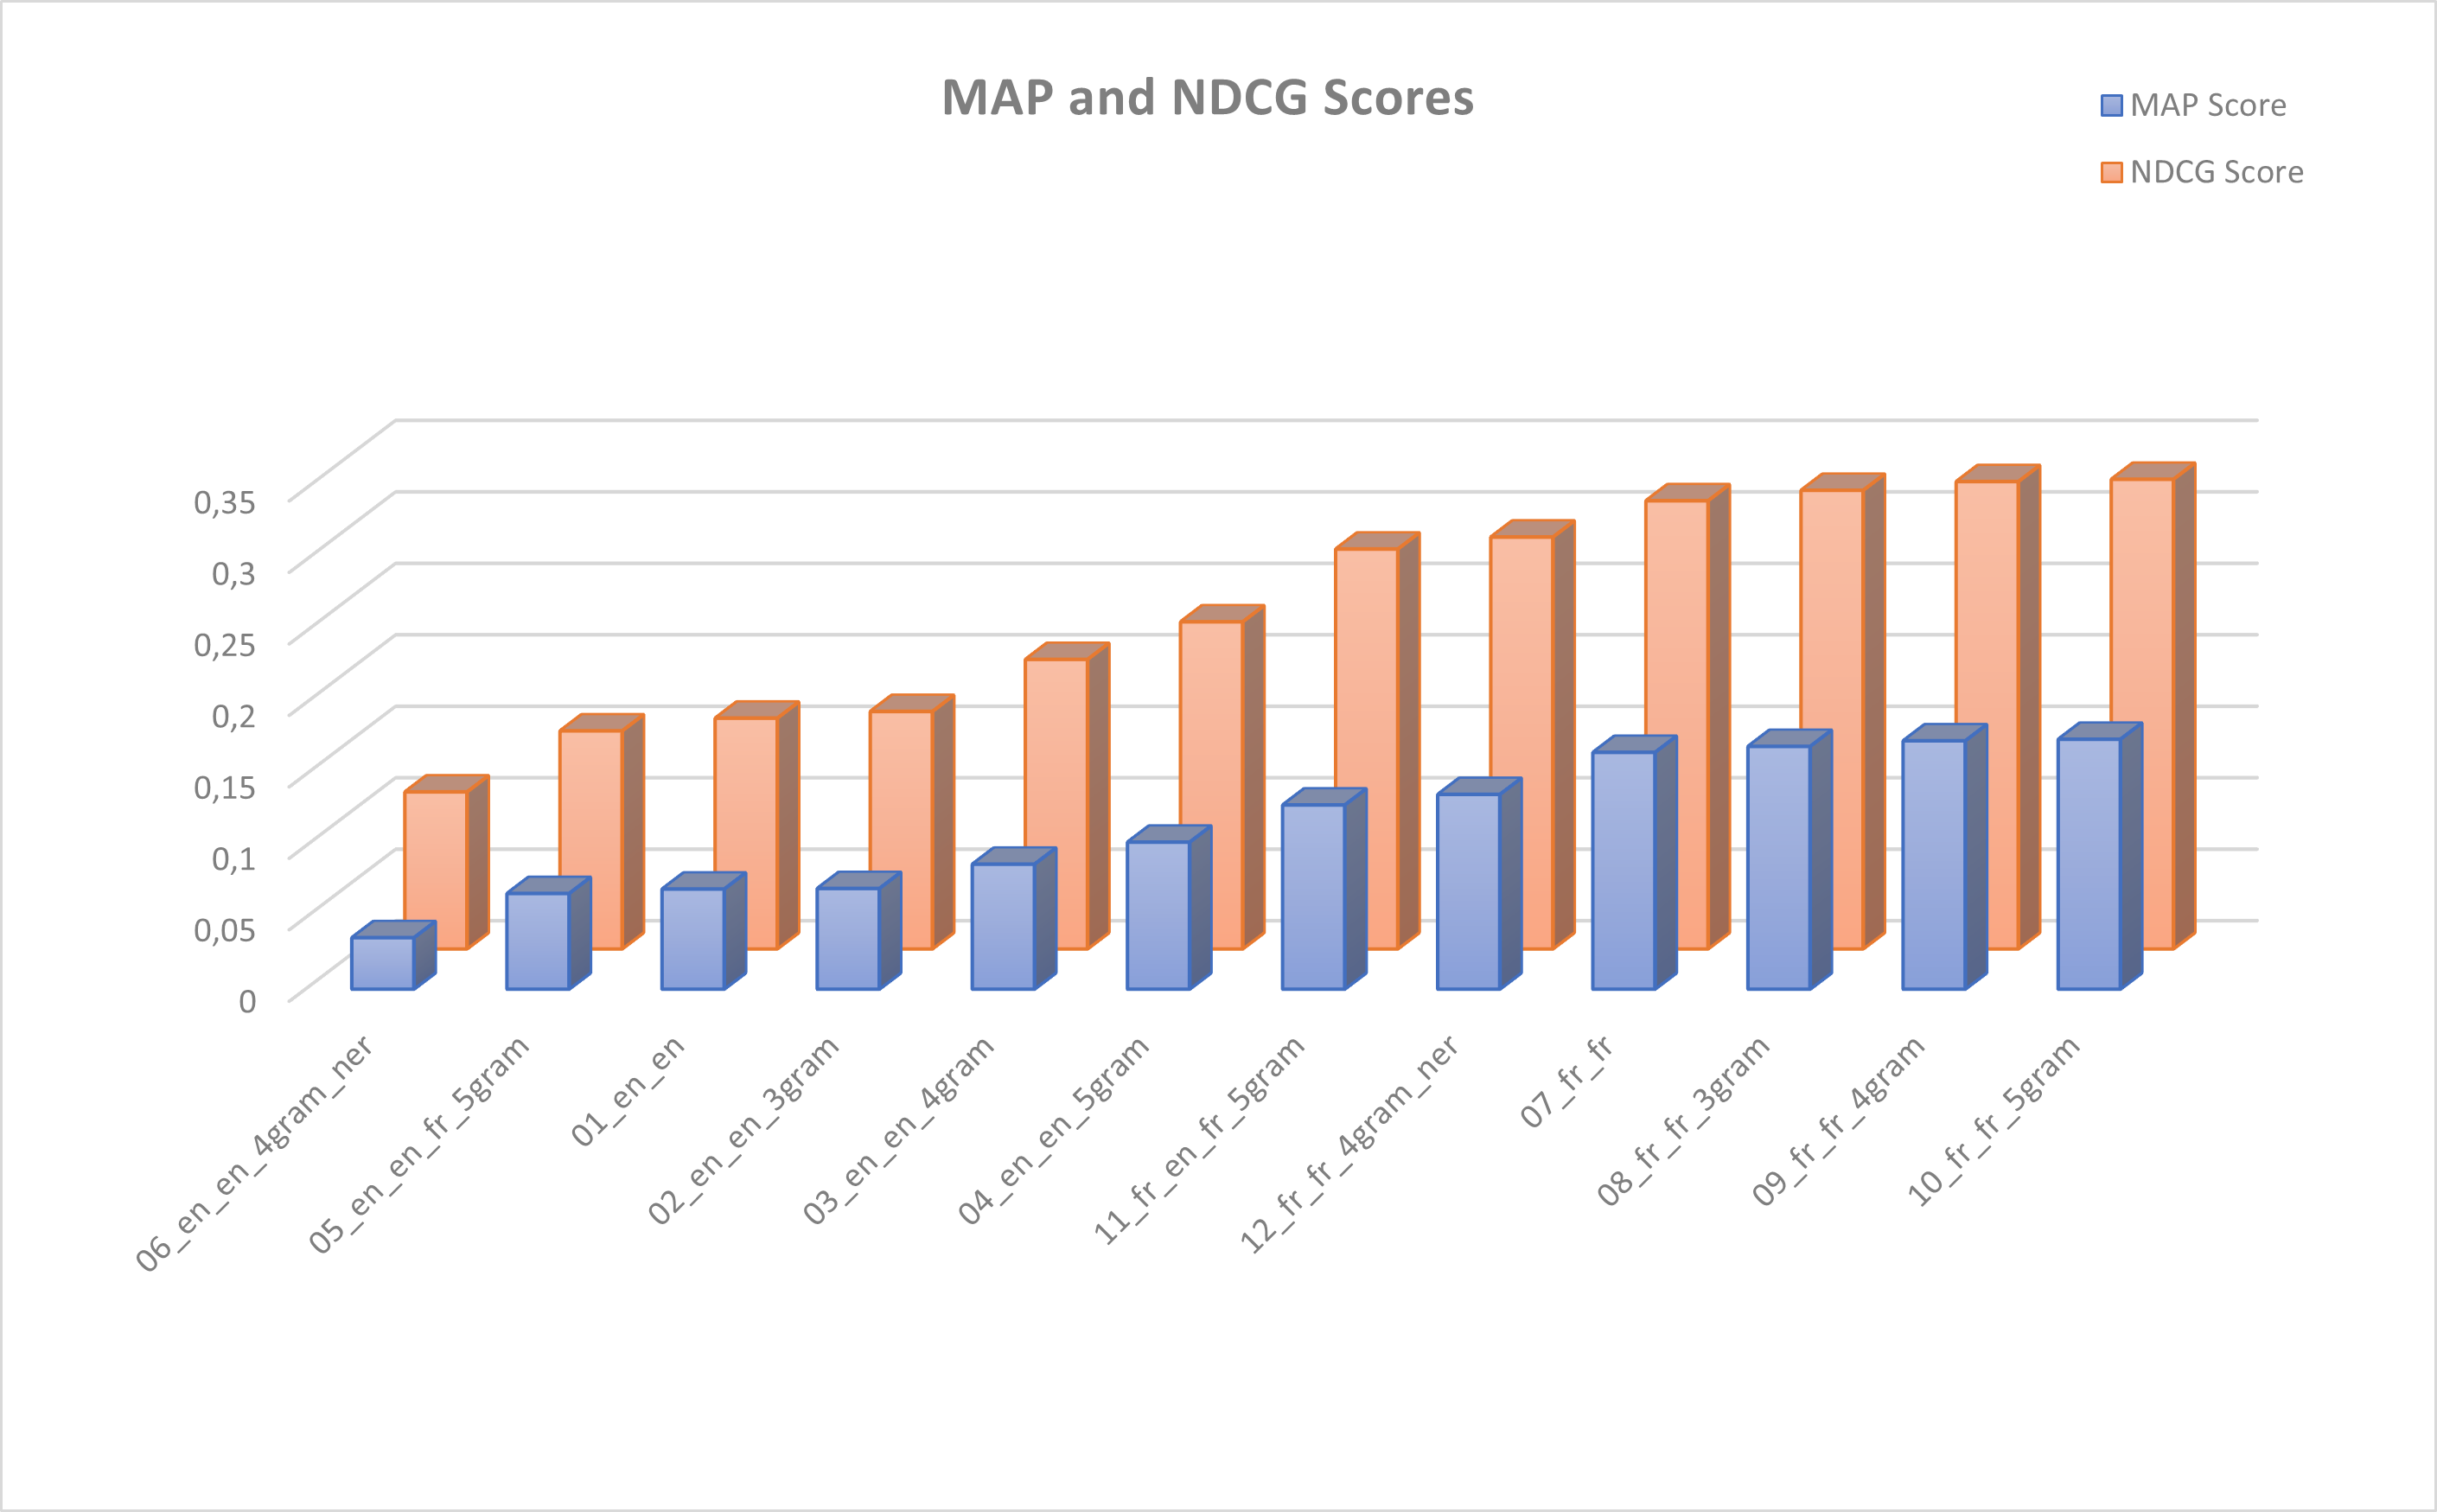
\includegraphics[width=0.6\textwidth]{figure/allScores}
%    \caption{All scores sorted by MAP score}
%    \label{fig:sorted_scores}
%\end{figure}

The analysis shows that the highest MAP score (0.1748) is achieved by \texttt{10\_fr\_fr\_5gram}, followed by
\texttt{09\_fr\_fr\_4gram} (0.1737),
\texttt{08\_fr\_fr\_3gram} (0.1698),
\texttt{07\_fr\_fr} (0.1656), and
\texttt{12\_fr\_fr\_4gram\_ner} (0.1362).
The lowest MAP score (0.0360) is obtained by \texttt{en\_en\_4gram\_ner}.

Similarly, the highest NDCG score (0.3285) belongs to \texttt{10\_fr\_fr\_5gram}, followed by
\texttt{09\_fr\_fr\_4gram} (0.3269),
\texttt{08\_fr\_fr\_3gram} (0.3208),
\texttt{07\_fr\_fr} (0.3135), and
\texttt{12\_fr\_fr\_4gram\_ner} (0.2881).
The lowest NDCG score (0.1098) corresponds to \texttt{en\_en\_4gram\_ner}.\\

Because of this, the five system submitted to CLEF have been (in order of importance): \texttt{10\_fr\_fr\_5gram},
\texttt{09\_fr\_fr\_4gram}, \texttt{08\_fr\_fr\_3gram}, \texttt{07\_fr\_fr}, \texttt{12\_fr\_fr\_4gram\_ner}.
Following the competition workflow, we created new indexes based on the test data and re-executed this top five runs.\\

% Ferro said that with this data we should only use the tables
%Here we can see a chart ranking of the five best scores, they are the runs that have been presented at CLEF:
%\begin{figure}[h!]
%    \centering
%    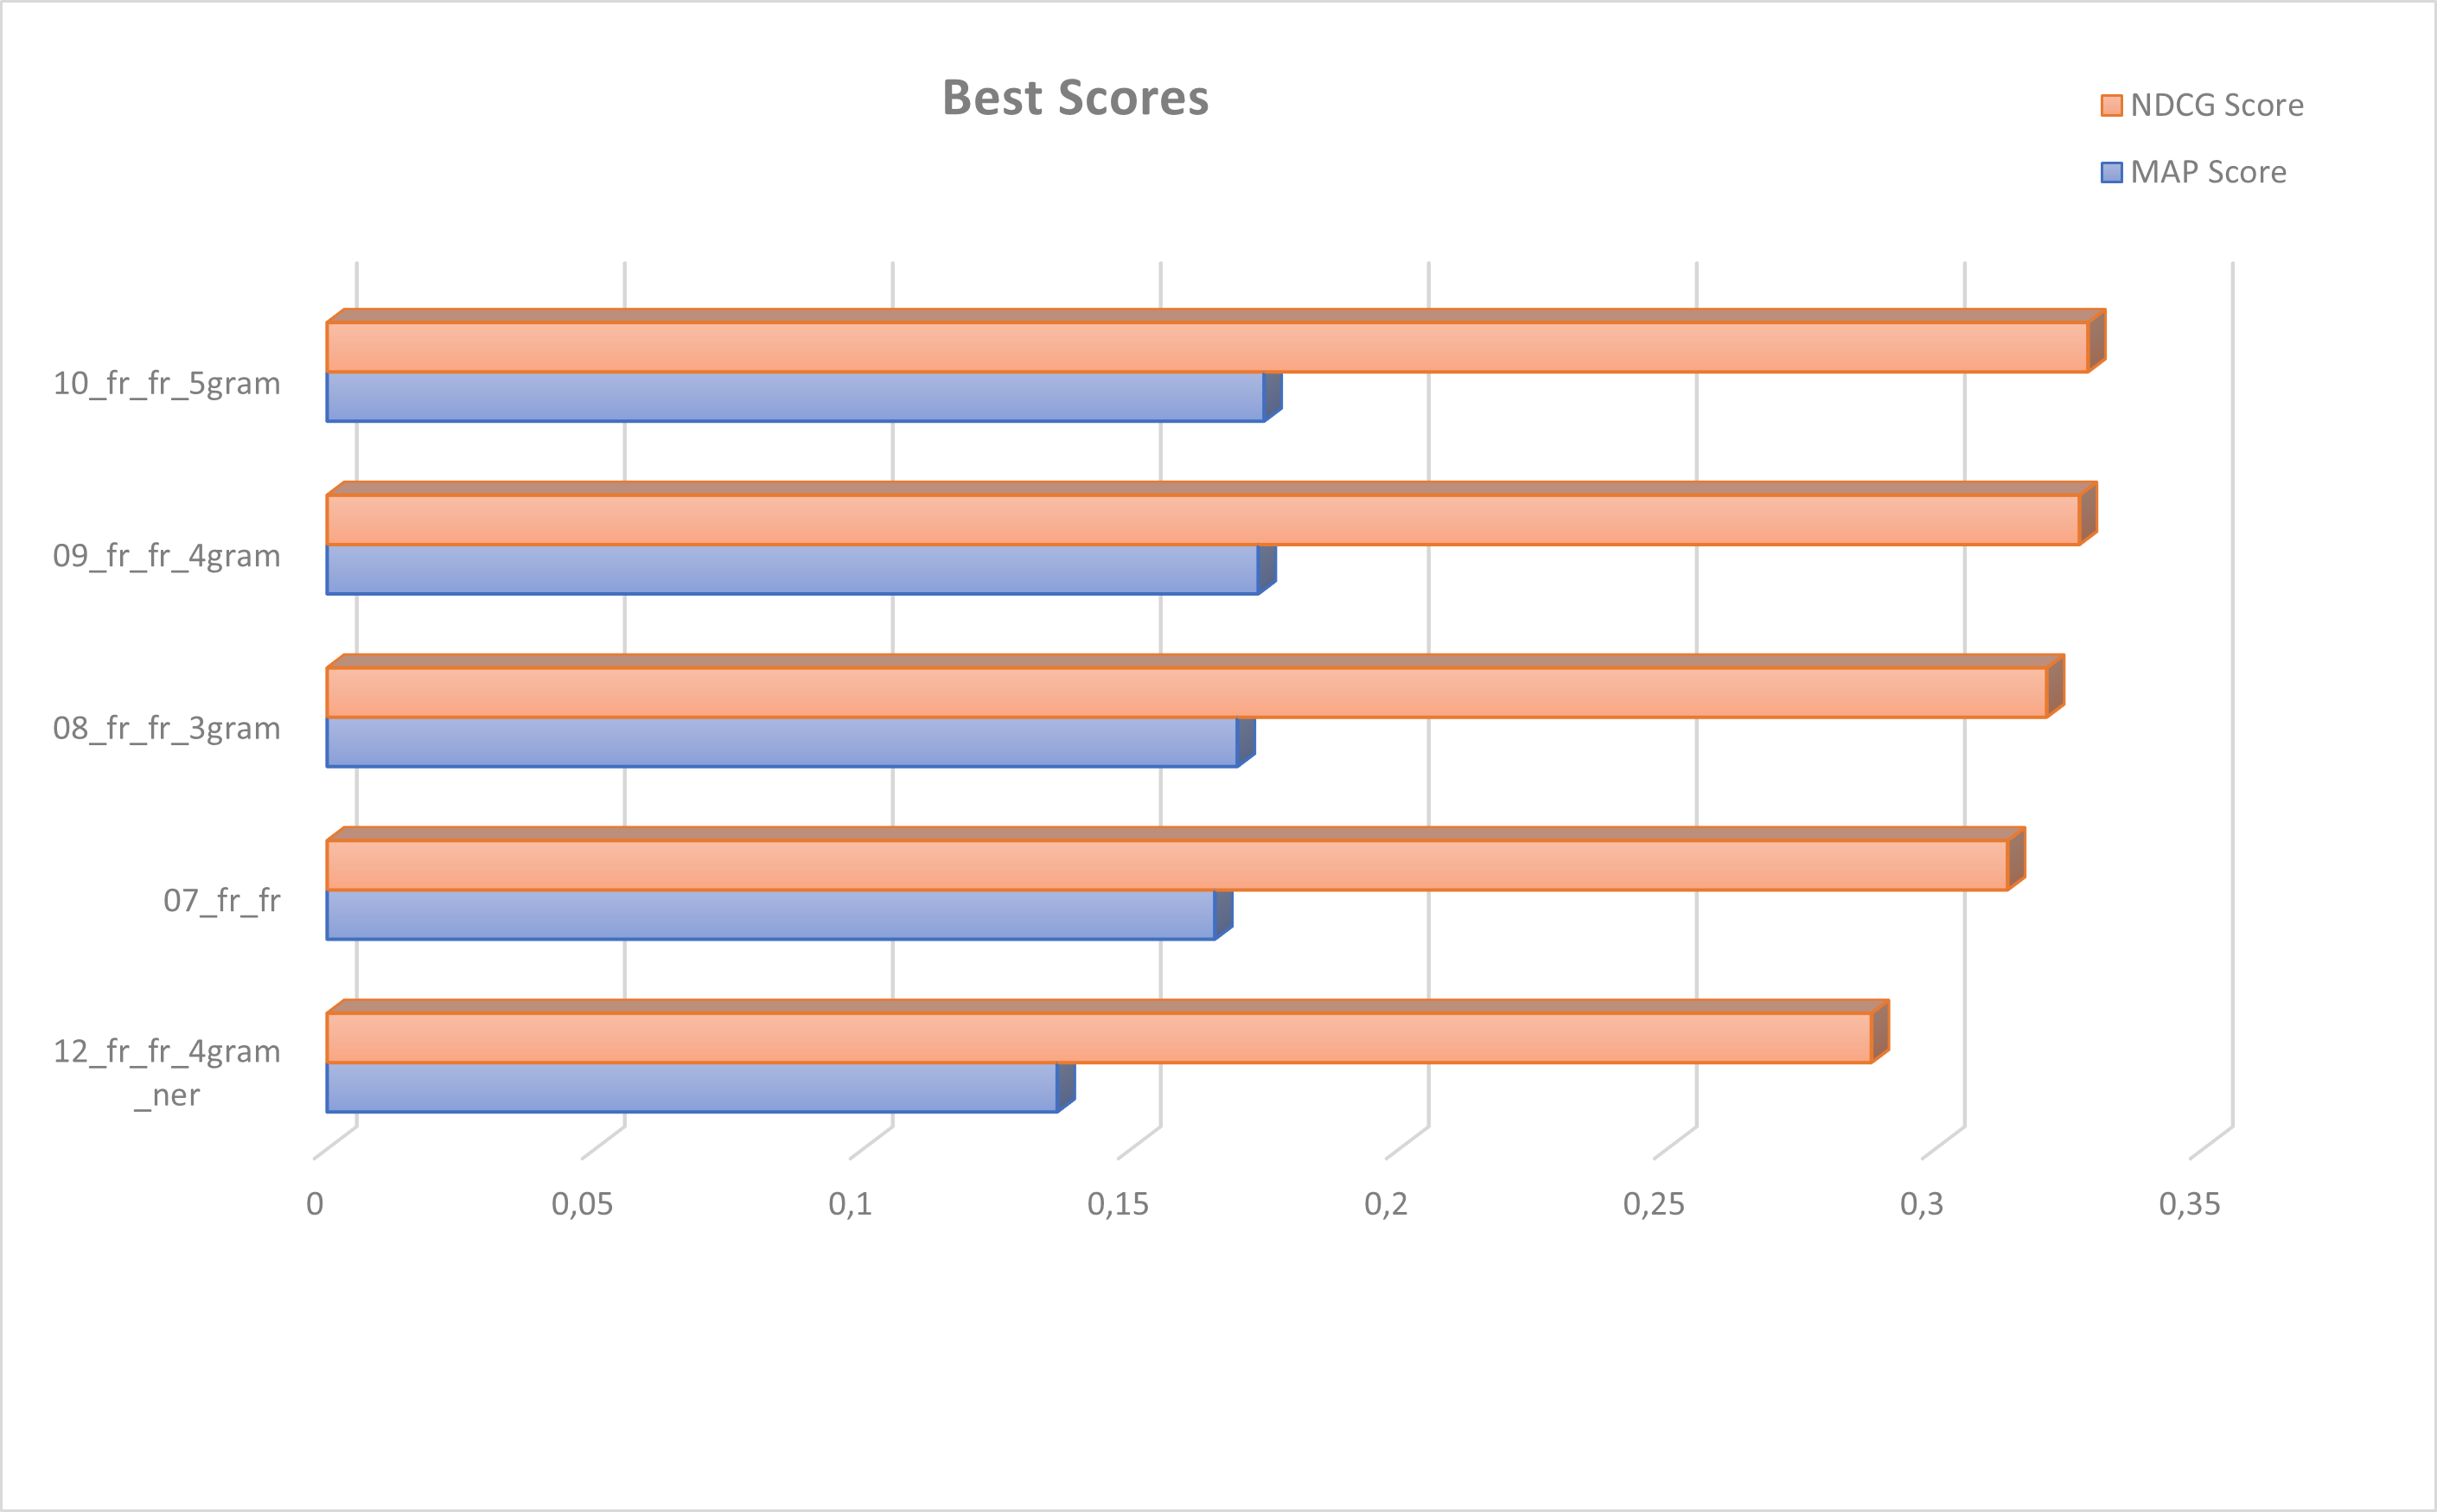
\includegraphics[width=0.6\textwidth]{figure/bestScores}
%    \caption{Best MAP and NDCG scores}
%    \label{fig:best_scores}
%\end{figure}

\section{Results and Discussion}
\label{sec:results}

\subsection{Short Term Test Data}

%TODO: Here we should include a table like the one we have previously done (MAP, nDCG, but also RnD) for the SHORT TERM runs, for the 5 systems submitted to CLEF.
%TODO: this is, we have to use trec_eval with the new qrels.txt file (for SHORT TERM) that have been submitted to CLEF on 22/5/2023 (see CLEF web page)

\subsection{Long Term Test Data}

%TODO: Here we should include a table like the one we have previously done (MAP, nDCG, but also RnD) for the LONG TERM runs, for the 5 systems submitted to CLEF.
%TODO: this is, we have to use trec_eval with the new qrels.txt file (for LONG TERM) that have been submitted to CLEF on 22/5/2023 (see CLEF web page)

\subsection{Anova 2 Analysis}

%TODO: here we have to do a 2 ways Anova for our five systems.

\section{Conclusions and Future Work}
\label{sec:conclusion}

In summary, the IR systems developed in this study followed the Parsing-Analyzer-Index-Search-Topic paradigm and utilized different methodologies, among which the following stand out: processing of English documents based on whitespace tokenization, the TERRIER stopword list, query expansion and stemming; processing of French documents based on whitespace tokenization, a stopword list and stemming; character N-grams of both versions concatenated; and NER information extraction using NLP techniques.\\

In terms of future work, there are several areas that could be explored to improve the effectiveness of the developed IR systems. Firstly, we could improve indexing methodologies, such as increasing the value of N in N-gram, as we have commented on in Section~\ref{sec:results}. Secondly, we could explore better NLP techniques to improve the accuracy of the IR systems, as NER turns out not to be very effective.\\

One last possible future work could be a machine-learning based IR system. This would be a more dynamic approach to IR systems, as it would be able to adapt to different types of queries and documents.

% TODO: Here we should add more conclusions taken from HW2

%% Define the bibliography file to be used
\bibliography{bibliography,proceedings}

\acrodef{3G}[3G]{Third Generation Mobile System}
\acrodef{5S}[5S]{Streams, Structures, Spaces, Scenarios, Societies}
\acrodef{AA}[AA]{Active Agreements}
\acrodef{AAAI}[AAAI]{Association for the Advancement of Artificial Intelligence}
\acrodef{AAL}[AAL]{Annotation Abstraction Layer}
\acrodef{AAM}[AAM]{Automatic Annotation Manager}
\acrodef{AAP}[AAP]{Average Average Precision}
\acrodef{ACLIA}[ACLIA]{Advanced Cross-Lingual Information Access}
\acrodef{ACM}[ACM]{Association for Computing Machinery}
\acrodef{AD}[AD]{Active Disagreements}
\acrodef{ADSL}[ADSL]{Asymmetric Digital Subscriber Line}
\acrodef{ADUI}[ADUI]{ADministrator User Interface}
\acrodef{AIP}[AIP]{Archival Information Package}
\acrodef{AJAX}[AJAX]{Asynchronous JavaScript Technology and \acs{XML}}
\acrodef{ALU}[ALU]{Aritmetic-Logic Unit}
\acrodef{AMUSID}[AMUSID]{Adaptive MUSeological IDentity-service}
\acrodef{ANOVA}[ANOVA]{ANalysis Of VAriance}
\acrodef{ANSI}[ANSI]{American National Standards Institute}
\acrodef{AP}[AP]{Average Precision}
\acrodef{APC}[APC]{AP Correlation}
\acrodef{API}[API]{Application Program Interface}
\acrodef{AR}[AR]{Address Register}
\acrodef{AS}[AS]{Annotation Service}
\acrodef{ASAP}[ASAP]{Adaptable Software Architecture Performance}
\acrodef{ASI}[ASI]{Annotation Service Integrator}
\acrodef{ASL}[ASL]{Achieved Significance Level}
\acrodef{ASM}[ASM]{Annotation Storing Manager}
\acrodef{ASR}[ASR]{Automatic Speech Recognition}
\acrodef{ASUI}[ASUI]{ASsessor User Interface}
\acrodef{ATIM}[ATIM]{Annotation Textual Indexing Manager}
\acrodef{AUC}[AUC]{Area Under the ROC Curve}
\acrodef{AUI}[AUI]{Administrative User Interface}
\acrodef{AWARE}[AWARE]{Assessor-driven Weighted Averages for Retrieval Evaluation}
\acrodef{BANKS-I}[BANKS-I]{Browsing ANd Keyword Searching I}
\acrodef{BANKS-II}[BANKS-II]{Browsing ANd Keyword Searching II}
\acrodef{BH}[BH]{Benjamini-Hochberg}
\acrodef{bpref}[bpref]{Binary Preference}
\acrodef{BNF}[BNF]{Backus and Naur Form}
\acrodef{BPM}[BPM]{Bejeweled Player Model}
\acrodef{BRICKS}[BRICKS]{Building Resources for Integrated Cultural Knowledge Services}
\acrodef{CAN}[CAN]{Content Addressable Netword}
\acrodef{CAS}[CAS]{Content-And-Structure}
\acrodef{CBSD}[CBSD]{Component-Based Software Developlement}
\acrodef{CBSE}[CBSE]{Component-Based Software Engineering}
\acrodef{CB-SPE}[CB-SPE]{Component-Based \acs{SPE}}
\acrodef{CD}[CD]{Collaboration Diagram}
\acrodef{CD}[CD]{Compact Disk}
\acrodef{CDF}[CDF]{Cumulative Density Function}
\acrodef{CENL}[CENL]{Conference of European National Librarians}
\acrodef{CIDOC CRM}[CIDOC CRM]{CIDOC Conceptual Reference Model}
\acrodef{CIR}[CIR]{Current Instruction Register}
\acrodef{CIRCO}[CIRCO]{Coordinated Information Retrieval Components Orchestration}
\acrodef{CG}[CG]{Cumulated Gain}
\acrodef{CL}[CL]{Curriculum Learning}
\acrodef{CL-ESA}[CL-ESA]{Cross-Lingual Explicit Semantic Analysis}
\acrodef{CLAIRE}[CLAIRE]{Combinatorial visuaL Analytics system for Information Retrieval Evaluation}
\acrodef{CLEF1}[CLEF]{Cross-Language Evaluation Forum}
\acrodef{CLEF}[CLEF]{Conference and Labs of the Evaluation Forum}
\acrodef{CLIR}[CLIR]{Cross Language Information Retrieval}
\acrodef{CM}[CM]{Continuation Methods}
\acrodef{CMS}[CMS]{Content Management System}
\acrodef{CMT}[CMT]{Campaign Management Tool}
\acrodef{CNR}[CNR]{Italian National Council of Research}
\acrodef{CO}[CO]{Content-Only}
\acrodef{COD}[COD]{Code On Demand}
\acrodef{CODATA}[CODATA]{Committee on Data for Science and Technology}
\acrodef{COLLATE}[COLLATE]{Collaboratory for Annotation Indexing and Retrieval of Digitized Historical Archive Material}
\acrodef{CP}[CP]{Characteristic Pattern}
\acrodef{CPE}[CPE]{Control Processor Element}
\acrodef{CPU}[CPU]{Central Processing Unit}
\acrodef{CQL}[CQL]{Contextual Query Language}
\acrodef{CRP}[CRP]{Cumulated Relative Position}
\acrodef{CRUD}[CRUD]{Create--Read--Update--Delete}
\acrodef{CS}[CS]{Characteristic Structure}
\acrodef{CSM}[CSM]{Campaign Storing Manager}
\acrodef{CSS}[CSS]{Cascading Style Sheets}
\acrodef{CTR}[CTR]{Click-Through Rate}
\acrodef{CU}[CU]{Control Unit}
\acrodef{CUI}[CUI]{Client User Interface}
\acrodef{CV}[CV]{Cross-Validation}
\acrodef{DAFFODIL}[DAFFODIL]{Distributed Agents for User-Friendly Access of Digital Libraries}
\acrodef{DAO}[DAO]{Data Access Object}
\acrodef{DARE}[DARE]{Drawing Adequate REpresentations}
\acrodef{DARPA}[DARPA]{Defense Advanced Research Projects Agency}
\acrodef{DAS}[DAS]{Distributed Annotation System}
\acrodef{DB}[DB]{DataBase}
\acrodef{DBMS}[DBMS]{DataBase Management System}
\acrodef{DC}[DC]{Dublin Core}
\acrodef{DCG}[DCG]{Discounted Cumulated Gain}
\acrodef{DCMI}[DCMI]{Dublin Core Metadata Initiative}
\acrodef{DCV}[DCV]{Document Cut--off Value}
\acrodef{DD}[DD]{Deployment Diagram}
\acrodef{DDC}[DDC]{Dewey Decimal Classification}
\acrodef{DDS}[DDS]{Direct Data Structure}
\acrodef{DF}[DF]{Degrees of Freedom}
\acrodef{DFI}[DFI]{Divergence From Independence}
\acrodef{DFR}[DFR]{Divergence From Randomness}
\acrodef{DHT}[DHT]{Distributed Hash Table}
\acrodef{DI}[DI]{Digital Image}
\acrodef{DIKW}[DIKW]{Data, Information, Knowledge, Wisdom}
\acrodef{DIL}[DIL]{\acs{DIRECT} Integration Layer}
\acrodef{DiLAS}[DiLAS]{Digital Library Annotation Service}
\acrodef{DIRECT}[DIRECT]{Distributed Information Retrieval Evaluation Campaign Tool}
\acrodef{DKMS}[DKMS]{Data and Knowledge Management System}
\acrodef{DL}[DL]{Digital Library}
\acrodefplural{DL}[DL]{Digital Libraries}
\acrodef{DLMS}[DLMS]{Digital Library Management System}
\acrodef{DLOG}[DL]{Description Logics}
\acrodef{DLS}[DLS]{Digital Library System}
\acrodef{DLSS}[DLSS]{Digital Library Service System}
\acrodef{DM}[DM]{Data Mining}
\acrodef{DO}[DO]{Digital Object}
\acrodef{DOI}[DOI]{Digital Object Identifier}
\acrodef{DOM}[DOM]{Document Object Model}
\acrodef{DoMDL}[DoMDL]{Document Model for Digital Libraries}
\acrodef{DP}[DP]{Discriminative Power}
\acrodef{DPBF}[DPBF]{Dynamic Programming Best-First}
\acrodef{DR}[DR]{Data Register}
\acrodef{DRIVER}[DRIVER]{Digital Repository Infrastructure Vision for European Research}
\acrodef{DTD}[DTD]{Document Type Definition}
\acrodef{DVD}[DVD]{Digital Versatile Disk}
\acrodef{EAC-CPF}[EAC-CPF]{Encoded Archival Context for Corporate Bodies, Persons, and Families}
\acrodef{EAD}[EAD]{Encoded Archival Description}
\acrodef{EAN}[EAN]{International Article Number}
\acrodef{EBU}[EBU]{Expected Browsing Utility}
\acrodef{ECD}[ECD]{Enhanced Contenty Delivery}
\acrodef{ECDL}[ECDL]{European Conference on Research and Advanced Technology for Digital Libraries}
\acrodef{EDM}[EDM]{Europeana Data Model}
\acrodef{EG}[EG]{Execution Graph}
\acrodef{ELDA}[ELDA]{Evaluation and Language resources Distribution Agency}
\acrodef{ELRA}[ELRA]{European Language Resources Association}
\acrodef{EM}[EM]{Expectation Maximization}
\acrodef{EMMA}[EMMA]{Extensible MultiModal Annotation}
\acrodef{EPROM}[EPROM]{Erasable Programmable \acs{ROM}}
\acrodef{EQNM}[EQNM]{Extended Queueing Network Model}
\acrodef{ER}[ER]{Entity--Relationship}
\acrodef{ERR}[ERR]{Expected Reciprocal Rank}
\acrodef{ERS}[ERS]{Empirical Relational System}
\acrodef{ESA}[ESA]{Explicit Semantic Analysis}
\acrodef{ESL}[ESL]{Expected Search Length}
\acrodef{ETL}[ETL]{Extract-Transform-Load}
\acrodef{FAST}[FAST]{Flexible Annotation Service Tool}
\acrodef{FDR}[FDR]{False Discovery Rate}
\acrodef{FIFO}[FIFO]{First-In / First-Out}
\acrodef{FIRE}[FIRE]{Forum for Information Retrieval Evaluation}
\acrodef{FN}[FN]{False Negative}
\acrodef{FNR}[FNR]{False Negative Rate}
\acrodef{FOAF}[FOAF]{Friend of a Friend}
\acrodef{FORESEE}[FORESEE]{FOod REcommentation sErvER}
\acrodef{FP}[FP]{False Positive}
\acrodef{FPR}[FPR]{False Positive Rate}
\acrodef{FWER}[FWER]{Family-wise Error Rate}
\acrodef{GIF}[GIF]{Graphics Interchange Format}
\acrodef{GIR}[GIR]{Geografic Information Retrieval}
\acrodef{GAP}[GAP]{Graded Average Precision}
\acrodef{GLM}[GLM]{General Linear Model}
\acrodef{GLMM}[GLMM]{General Linear Mixed Model}
\acrodef{GMAP}[GMAP]{Geometric Mean Average Precision}
\acrodef{GoP}[GoP]{Grid of Points}
\acrodef{GPRS}[GPRS]{General Packet Radio Service}
\acrodef{gP}[gP]{Generalized Precision}
\acrodef{gR}[gR]{Generalized Recall}
\acrodef{gRBP}[gRBP]{Graded Rank-Biased Precision}
\acrodef{GT}[GT]{Generalizability Theory}
\acrodef{GTIN}[GTIN]{Global Trade Item Number}
\acrodef{GUI}[GUI]{Graphical User Interface}
\acrodef{GW}[GW]{Gateway}
\acrodef{HCI}[HCI]{Human Computer Interaction}
\acrodef{HDS}[HDS]{Hybrid Data Structure}
\acrodef{HIR}[HIR]{Hypertext Information Retrieval}
\acrodef{HIT}[HIT]{Human Intelligent Task}
\acrodef{HITS}[HITS]{Hyperlink-Induced Topic Search}
\acrodef{HMM}[HMM]{Hidden Markov Model}
\acrodef{HTML}[HTML]{HyperText Markup Language}
\acrodef{HTTP}[HTTP]{HyperText Transfer Protocol}
\acrodef{HSD}[HSD]{Honestly Significant Difference}
\acrodef{ICA}[ICA]{International Council on Archives}
\acrodef{ICSU}[ICSU]{International Council for Science}
\acrodef{IDF}[IDF]{Inverse Document Frequency}
\acrodef{IDS}[IDS]{Inverse Data Structure}
\acrodef{IEEE}[IEEE]{Institute of Electrical and Electronics Engineers}
\acrodef{IEI}[IEI]{Istituto della Enciclopedia Italiana fondata da Giovanni Treccani}
\acrodef{IETF}[IETF]{Internet Engineering Task Force}
\acrodef{IIR}[IIR]{Interactive Information Retrieval}
\acrodef{IMS}[IMS]{Information Management System}
\acrodef{IMSPD}[IMS]{Information Management Systems Research Group}
\acrodef{indAP}[indAP]{Induced Average Precision}
\acrodef{infAP}[infAP]{Inferred Average Precision}
\acrodef{INEX}[INEX]{INitiative for the Evaluation of \acs{XML} Retrieval}
\acrodef{INS-M}[INS-M]{Inverse Set Data Model}
\acrodef{INTR}[INTR]{Interrupt Register}
\acrodef{IP}[IP]{Internet Protocol}
\acrodef{IPSA}[IPSA]{Imaginum Patavinae Scientiae Archivum}
\acrodef{IR}[IR]{Information Retrieval}
\acrodef{IRON}[IRON]{Information Retrieval ON}
\acrodef{IRON2}[IRON$^2$]{Information Retrieval On aNNotations}
\acrodef{IRON-SAT}[IRON-SAT]{\acs{IRON} - Statistical Analysis Tool}
\acrodef{IRS}[IRS]{Information Retrieval System}
\acrodef{ISAD(G)}[ISAD(G)]{International Standard for Archival Description (General)}
\acrodef{ISBN}[ISBN]{International Standard Book Number}
\acrodef{ISIS}[ISIS]{Interactive SImilarity Search}
\acrodef{ISJ}[ISJ]{Interactive Searching and Judging}
\acrodef{ISO}[ISO]{International Organization for Standardization}
\acrodef{ITU}[ITU]{International Telecommunication Union }
\acrodef{ITU-T}[ITU-T]{Telecommunication Standardization Sector of \acs{ITU}}
\acrodef{IV}[IV]{Information Visualization}
\acrodef{JAN}[JAN]{Japanese Article Number}
\acrodef{JDBC}[JDBC]{Java DataBase Connectivity}
\acrodef{JMB}[JMB]{Java--Matlab Bridge}
\acrodef{JPEG}[JPEG]{Joint Photographic Experts Group}
\acrodef{JSON}[JSON]{JavaScript Object Notation}
\acrodef{JSP}[JSP]{Java Server Pages}
\acrodef{JTE}[JTE]{Java-Treceval Engine}
\acrodef{KDE}[KDE]{Kernel Density Estimation}
\acrodef{KLD}[KLD]{Kullback-Leibler Divergence}
\acrodef{KLAPER}[KLAPER]{Kernel LAnguage for PErformance and Reliability analysis}
\acrodef{LAM}[LAM]{Libraries, Archives, and Museums}
\acrodef{LAM2}[LAM]{Logistic Average Misclassification}
\acrodef{LAN}[LAN]{Local Area Network}
\acrodef{LD}[LD]{Linked Data}
\acrodef{LEAF}[LEAF]{Linking and Exploring Authority Files}
\acrodef{LIDO}[LIDO]{Lightweight Information Describing Objects}
\acrodef{LIFO}[LIFO]{Last-In / First-Out}
\acrodef{LM}[LM]{Language Model}
\acrodef{LMT}[LMT]{Log Management Tool}
\acrodef{LOD}[LOD]{Linked Open Data}
\acrodef{LODE}[LODE]{Linking Open Descriptions of Events}
\acrodef{LpO}[LpO]{Leave-$p$-Out}
\acrodef{LRM}[LRM]{Local Relational Model}
\acrodef{LRU}[LRU]{Last Recently Used}
\acrodef{LS}[LS]{Lexical Signature}
\acrodef{LSM}[LSM]{Log Storing Manager}
\acrodef{LtR}[LtR]{Learning to Rank}
\acrodef{LUG}[LUG]{Lexical Unit Generator}
\acrodef{MA}[MA]{Mobile Agent}
\acrodef{MA}[MA]{Moving Average}
\acrodef{MACS}[MACS]{Multilingual ACcess to Subjects}
\acrodef{MADCOW}[MADCOW]{Multimedia Annotation of Digital Content Over the Web}
\acrodef{MAD}[MAD]{Mean Assessed Documents}
\acrodef{MADP}[MADP]{Mean Assessed Documents Precision}
\acrodef{MADS}[MADS]{Metadata Authority Description Standard}
\acrodef{MAP}[MAP]{Mean Average Precision}
\acrodef{MARC}[MARC]{Machine Readable Cataloging}
\acrodef{MATTERS}[MATTERS]{MATlab Toolkit for Evaluation of information Retrieval Systems}
\acrodef{MDA}[MDA]{Model Driven Architecture}
\acrodef{MDD}[MDD]{Model-Driven Development}
\acrodef{METS}[METS]{Metadata Encoding and Transmission Standard}
\acrodef{MIDI}[MIDI]{Musical Instrument Digital Interface}
\acrodef{MIME}[MIME]{Multipurpose Internet Mail Extensions}
\acrodef{ML}[ML]{Machine Learning}
\acrodef{MLE}[MLE]{Maximum Likelihood Estimation}
\acrodef{MLIA}[MLIA]{MultiLingual Information Access}
\acrodef{MM}[MM]{Machinery Model}
\acrodef{MMU}[MMU]{Memory Management Unit}
\acrodef{MODS}[MODS]{Metadata Object Description Schema}
\acrodef{MOF}[MOF]{Meta-Object Facility}
\acrodef{MP}[MP]{Markov Precision}
\acrodef{MPEG}[MPEG]{Motion Picture Experts Group}
\acrodef{MRD}[MRD]{Machine Readable Dictionary}
\acrodef{MRF}[MRF]{Markov Random Field}
\acrodef{MRR}[MRR]{Mean Reciprocal Rank}
\acrodef{MS}[MS]{Mean Squares}
\acrodef{MSAC}[MSAC]{Multilingual Subject Access to Catalogues}
\acrodef{MSE}[MSE]{Mean Square Error}
\acrodef{MT}[MT]{Machine Translation}
\acrodef{MV}[MV]{Majority Vote}
\acrodef{MVC}[MVC]{Model-View-Controller}
\acrodef{NACSIS}[NACSIS]{NAtional Center for Science Information Systems}
\acrodef{NAP}[NAP]{Network processors Applications Profile}
\acrodef{NCP}[NCP]{Normalized Cumulative Precision}
\acrodef{nCG}[nCG]{Normalized Cumulated Gain}
\acrodef{nCRP}[nCRP]{Normalized Cumulated Relative Position}
\acrodef{nDCG}[nDCG]{Normalized Discounted Cumulated Gain}
\acrodef{nMCG}[nMCG]{Normalized Markov Cumulated Gain}
\acrodef{NESTOR}[NESTOR]{NEsted SeTs for Object hieRarchies}
\acrodef{NEXI}[NEXI]{Narrowed Extended XPath I}
\acrodef{NII}[NII]{National Institute of Informatics}
\acrodef{NISO}[NISO]{National Information Standards Organization}
\acrodef{NIST}[NIST]{National Institute of Standards and Technology}
\acrodef{NLP}[NLP]{Natural Language Processing}
\acrodef{NN}[NN]{Neural Network}
\acrodef{NP}[NP]{Network Processor}
\acrodef{NR}[NR]{Normalized Recall}
\acrodef{NRS}[NRS]{Numerical Relational System}
\acrodef{NS-M}[NS-M]{Nested Set Model}
\acrodef{NTCIR}[NTCIR]{NII Testbeds and Community for Information access Research}
\acrodef{OAI}[OAI]{Open Archives Initiative}
\acrodef{OAI-ORE}[OAI-ORE]{Open Archives Initiative Object Reuse and Exchange}
\acrodef{OAI-PMH}[OAI-PMH]{Open Archives Initiative Protocol for Metadata Harvesting}
\acrodef{OAIS}[OAIS]{Open Archival Information System}
\acrodef{OC}[OC]{Operation Code}
\acrodef{OCLC}[OCLC]{Online Computer Library Center}
\acrodef{OMG}[OMG]{Object Management Group}
\acrodef{OO}[OO]{Object Oriented}
\acrodef{OODB}[OODB]{Object-Oriented \acs{DB}}
\acrodef{OODBMS}[OODBMS]{Object-Oriented \acs{DBMS}}
\acrodef{OPAC}[OPAC]{Online Public Access Catalog}
\acrodef{OQL}[OQL]{Object Query Language}
\acrodef{ORP}[ORP]{Open Relevance Project}
\acrodef{OSIRIS}[OSIRIS]{Open Service Infrastructure for Reliable and Integrated process Support}
\acrodef{P}[P]{Precision}
\acrodef{P2P}[P2P]{Peer-To-Peer}
\acrodef{PA}[PA]{Passive Agreements}
\acrodef{PAMT}[PAMT]{Pool-Assessment Management Tool}
\acrodef{PASM}[PASM]{Pool-Assessment Storing Manager}
\acrodef{PC}[PC]{Program Counter}
\acrodef{PCP}[PCP]{Pre-Commercial Procurement}
\acrodef{PCR}[PCR]{Peripherical Command Register}
\acrodef{PD}[PD]{Passive Disagreements}
\acrodef{PDA}[PDA]{Personal Digital Assistant}
\acrodef{PDF}[PDF]{Probability Density Function}
\acrodef{PDR}[PDR]{Peripherical Data Register}
\acrodef{PIR}[PIR]{Personalized Information Retrieval}
\acrodef{POI}[POI]{\acs{PURL}-based Object Identifier}
\acrodef{PoS}[PoS]{Part of Speech}
\acrodef{PAA}[PAA]{Proportion of Active Agreements}
\acrodef{PPA}[PPA]{Proportion of Passive Agreements}
\acrodef{PPE}[PPE]{Programmable Processing Engine}
\acrodef{PREFORMA}[PREFORMA]{PREservation FORMAts for culture information/e-archives}
\acrodef{PRIMAD}[PRIMAD]{Platform, Research goal, Implementation, Method, Actor, and Data}
\acrodef{PRIMAmob-UML}[PRIMAmob-UML]{mobile \acs{PRIMA-UML}}
\acrodef{PRIMA-UML}[PRIMA-UML]{PeRformance IncreMental vAlidation in \acs{UML}}
\acrodef{PROM}[PROM]{Programmable \acs{ROM}}
\acrodef{PROMISE}[PROMISE]{Participative Research labOratory  for Multimedia and Multilingual Information Systems Evaluation}
\acrodef{pSQL}[pSQL]{propagate \acs{SQL}}
\acrodef{PUI}[PUI]{Participant User Interface}
\acrodef{PURL}[PURL]{Persistent \acs{URL}}
\acrodef{QA}[QA]{Question Answering}
\acrodef{QE}[QE]{Query Expansion}
\acrodef{QoS-UML}[QoS-UML]{\acs{UML} Profile for QoS and Fault Tolerance}
\acrodef{QPA}[QPA]{Query Performance Analyzer}
\acrodef{QPP}[QPP]{Query Performance Prediction}
\acrodef{R}[R]{Recall}
\acrodef{RAM}[RAM]{Random Access Memory}
\acrodef{RAMM}[RAM]{Random Access Machine}
\acrodef{RBO}[RBO]{Rank-Biased Overlap}
\acrodef{RBP}[RBP]{Rank-Biased Precision}
\acrodef{RBTO}[RBTO]{Rank-Based Total Order}
\acrodef{RDBMS}[RDBMS]{Relational \acs{DBMS}}
\acrodef{RDF}[RDF]{Resource Description Framework}
\acrodef{REST}[REST]{REpresentational State Transfer}
\acrodef{REV}[REV]{Remote Evaluation}
\acrodef{RF}[RF]{Relevance Feedback}
\acrodef{RFC}[RFC]{Request for Comments}
\acrodef{RIA}[RIA]{Reliable Information Access}
\acrodef{RMSE}[RMSE]{Root Mean Square Error}
\acrodef{RMT}[RMT]{Run Management Tool}
\acrodef{ROM}[ROM]{Read Only Memory}
\acrodef{ROMIP}[ROMIP]{Russian Information Retrieval Evaluation Seminar}
\acrodef{RoMP}[RoMP]{Rankings of Measure Pairs}
\acrodef{RoS}[RoS]{Rankings of Systems}
\acrodef{RP}[RP]{Relative Position}
\acrodef{RR}[RR]{Reciprocal Rank}
\acrodef{RSM}[RSM]{Run Storing Manager}
\acrodef{RST}[RST]{Rhetorical Structure Theory}
\acrodef{RSV}[RSV]{Retrieval Status Value}
\acrodef{RT-UML}[RT-UML]{\acs{UML} Profile for Schedulability, Performance and Time}
\acrodef{SA}[SA]{Software Architecture}
\acrodef{SAL}[SAL]{Storing Abstraction Layer}
\acrodef{SAMT}[SAMT]{Statistical Analysis Management Tool}
\acrodef{SAN}[SAN]{Sistema Archivistico Nazionale}
\acrodef{SASM}[SASM]{Statistical Analysis Storing Manager}
\acrodef{SBTO}[SBTO]{Set-Based Total Order}
\acrodef{SD}[SD]{Sequence Diagram}
\acrodef{SE}[SE]{Search Engine}
\acrodef{SEBD}[SEBD]{Convegno Nazionale su Sistemi Evoluti per Basi di Dati}
\acrodef{SEM}[SEM]{Standard Error of the Mean}
\acrodef{SERP}[SERP]{Search Engine Result Page}
\acrodef{SFT}[SFT]{Satisfaction--Frustration--Total}
\acrodef{SIL}[SIL]{Service Integration Layer}
\acrodef{SIP}[SIP]{Submission Information Package}
\acrodef{SKOS}[SKOS]{Simple Knowledge Organization System}
\acrodef{SM}[SM]{Software Model}
\acrodef{SME}[SME]{Statistics--Metrics-Experiments}
\acrodef{SMART}[SMART]{System for the Mechanical Analysis and Retrieval of Text}
\acrodef{SoA}[SoA]{Service-oriented Architectures}
\acrodef{SOA}[SOA]{Strength of Association}
\acrodef{SOAP}[SOAP]{Simple Object Access Protocol}
\acrodef{SOM}[SOM]{Self-Organizing Map}
\acrodef{SPARQL}[SPARQL]{Simple Protocol and RDF Query Language}
\acrodef{SPE}[SPE]{Software Performance Engineering}
\acrodef{SPINA}[SPINA]{Superimposed Peer Infrastructure for iNformation Access}
\acrodef{SPLIT}[SPLIT]{Stemming Program for Language Independent Tasks}
\acrodef{SPOOL}[SPOOL]{Simultaneous Peripheral Operations On Line}
\acrodef{SQL}[SQL]{Structured Query Language}
\acrodef{SR}[SR]{Sliding Ratio}
\acrodef{sRBP}[sRBP]{Session Rank Biased Precision}
\acrodef{SRU}[SRU]{Search/Retrieve via \acs{URL}}
\acrodef{SS}[SS]{Sum of Squares}
\acrodef{SSD}[s.s.d.]{statistically significantly different}
\acrodef{SSTF}[SSTF]{Shortest Seek Time First}
\acrodef{STAR}[STAR]{Steiner-Tree Approximation in Relationship graphs}
\acrodef{STON}[STON]{STemming ON}
\acrodef{SVM}[SVM]{Support Vector Machine}
\acrodef{TAC}[TAC]{Text Analysis Conference}
\acrodef{TBG}[TBG]{Time-Biased Gain}
\acrodef{TCP}[TCP]{Transmission Control Protocol}
\acrodef{TEL}[TEL]{The European Library}
\acrodef{TERRIER}[TERRIER]{TERabyte RetrIEveR}
\acrodef{TF}[TF]{Term Frequency}
\acrodef{TFR}[TFR]{True False Rate}
\acrodef{TLD}[TLD]{Top Level Domain}
\acrodef{TME}[TME]{Topics--Metrics-Experiments}
\acrodef{TN}[TN]{True Negative}
\acrodef{TO}[TO]{Transfer Object}
\acrodef{TP}[TP]{True Positve}
\acrodef{TPR}[TPR]{True Positive Rate}
\acrodef{TRAT}[TRAT]{Text Relevance Assessing Task}
\acrodef{TREC}[TREC]{Text REtrieval Conference}
\acrodef{TRECVID}[TRECVID]{TREC Video Retrieval Evaluation}
\acrodef{TTL}[TTL]{Time-To-Live}
\acrodef{UCD}[UCD]{Use Case Diagram}
\acrodef{UDC}[UDC]{Universal Decimal Classification}
\acrodef{uGAP}[uGAP]{User-oriented Graded Average Precision}
\acrodef{UI}[UI]{User Interface}
\acrodef{UML}[UML]{Unified Modeling Language}
\acrodef{UMT}[UMT]{User Management Tool}
\acrodef{UMTS}[UMTS]{Universal Mobile Telecommunication System}
\acrodef{UoM}[UoM]{Utility-oriented Measurement}
\acrodef{UPC}[UPC]{Universal Product Code}
\acrodef{URI}[URI]{Uniform Resource Identifier}
\acrodef{URL}[URL]{Uniform Resource Locator}
\acrodef{URN}[URN]{Uniform Resource Name}
\acrodef{USM}[USM]{User Storing Manager}
\acrodef{VA}[VA]{Visual Analytics}
\acrodef{VAIRE}[VAIR\"{E}]{Visual Analytics for Information Retrieval Evaluation}
\acrodef{VATE}[VATE$^2$]{Visual Analytics Tool for Experimental Evaluation}
\acrodef{VIRTUE}[VIRTUE]{Visual Information Retrieval Tool for Upfront Evaluation}
\acrodef{VD}[VD]{Virtual Document}
\acrodef{VDM}[VDM]{Visual Data Mining}
\acrodef{VIAF}[VIAF]{Virtual International Authority File}
\acrodef{VIM}[VIM]{International Vocabulary of Metrology}
\acrodef{VL}[VL]{Visual Language}
\acrodef{VoIP}[VoIP]{Voice over IP}
\acrodef{VS}[VS]{Visual Sentence}
\acrodef{W3C}[W3C]{World Wide Web Consortium}
\acrodef{WAN}[WAN]{Wide Area Network}
\acrodef{WHO}[WHO]{World Health Organization}
\acrodef{WLAN}[WLAN]{Wireless \acs{LAN}}
\acrodef{WP}[WP]{Work Package}
\acrodef{WS}[WS]{Web Services}
\acrodef{WSD}[WSD]{Word Sense Disambiguation}
\acrodef{WSDL}[WSDL]{Web Services Description Language}
\acrodef{WWW}[WWW]{World Wide Web}
\acrodef{XMI}[XMI]{\acs{XML} Metadata Interchange}
\acrodef{XML}[XML]{eXtensible Markup Language}
\acrodef{XPath}[XPath]{XML Path Language}
\acrodef{XSL}[XSL]{eXtensible Stylesheet Language}
\acrodef{XSL-FO}[XSL-FO]{\acs{XSL} Formatting Objects}
\acrodef{XSLT}[XSLT]{\acs{XSL} Transformations}
\acrodef{YAGO}[YAGO]{Yet Another Great Ontology}
\acrodef{YASS}[YASS]{Yet Another Suffix Stripper}



\end{document}
